\documentclass[a4paper]{report}

% Setup layout
\usepackage{geometry}
\geometry{paper=a4paper}

% Font setup
\usepackage[T1]{fontenc}
\usepackage[utf8]{inputenx}
\usepackage{palatino}
\usepackage{mathpazo}
\usepackage{microtype}
\renewcommand*\ttdefault{txtt}

% Language setup
\usepackage[czech,english]{babel}

% Setup hyperlinks in PDF
\usepackage[
  pdftex,
  breaklinks=true,
  pdfborder={0 0 0}
]{hyperref}

% Glossaries
\usepackage[sort=def, xindy, nonumberlist]{glossaries}
\usepackage{glossary-long}
\makeglossaries

% Other includes
\usepackage{url}
\usepackage{paralist}
\usepackage{parcolumns}
\usepackage{xcolor}
\usepackage{graphicx}
\usepackage{longtable}
\usepackage{multirow}
\usepackage{tikz}

% If then else
\usepackage{ifthen}

% Code listing
\usepackage{verbatim}
\usepackage{listingsutf8}
\usepackage{showexpl}
\lstset{
  escapechar=\⠶
}

% Bibliography
\usepackage[nottoc]{tocbibind}
\bibliographystyle{elsarticle-num}

% Command \provideenvironment and \providecounter
\makeatletter
\def\provideenvironment{\@star@or@long\provide@environment}
\def\provide@environment#1{%
        \@ifundefined{#1}%
                {\def\reserved@a{\newenvironment{#1}}}%
                {\def\reserved@a{\renewenvironment{dummy@environ}}}%
        \reserved@a
}
\def\dummy@environ{}
\makeatother
\makeatletter
\newcommand*\providecounter[1]{%
  \@ifundefined{c@#1}%
    {\@definecounter{#1}}%
    {}%
}
\makeatother

% Command \todo
\newcommand{\todo}[1]{%
\def\empty{}%
\def\prvniparametr{#1}%
\ifx\prvniparametr\empty%
\begingroup\small\tt\textcolor{red}{\noindent\textbf{TODO}}\endgroup
\else%
\begingroup\small\tt\textcolor{red}{\noindent\textbf{TODO:}\ #1}\endgroup
\fi%
}

% Code inline
\lstdefinestyle{lstStyleShort}{
  breaklines=true,
  breakatwhitespace=true,
  breakautoindent=true,
}
\newcommand{\code}[1]{\textbf{\small\texttt{#1}}}

% Document title page
\author{Petr Holub, Jan Růžička, Miloš Liška, Martin Šrom, Ondřej Pavelka, Ondřej Bouda}
\date{\copyright~CESNET~z.\,s.\,p.\,o.\\2012}

%%%%%%%%%%%%%%%%%%%%%%%%%%%%%%%%%%%%%%%%%%%%%%%%%%%%%%%%%%%%%%%%%%%%%%%%%%%%%%%%
% Entity example (type, name, comment)
\lstnewenvironment{ObjectCode}[3]{%
    \removelastskip
    \vskip 3mm
    \lstset{
      aboveskip=0pt,
      belowskip=0pt,    
      xleftmargin=8pt,
      basicstyle=\fontfamily{txtt}\selectfont,
      keywordstyle=\fontseries{b}\selectfont,
    }
    \minipage{\textwidth}
    \advance\leftmargini -3mm \quote
    \footnotesize\ttfamily #2 = \ifx&#1&\else\textbf{#1} \fi{}\{
    \ifx&#3& \else {\color{gray}// #3} \fi
}{%    
    \vspace*{-4pt}
    \footnotesize\ttfamily \}
    \endquote
    \endminipage
    \vskip 3mm
}




\usepackage{titlesec}

\titleformat{\chapter}[display]
    {\normalfont\huge\bfseries}{\chaptertitlename\ \thechapter}{20pt}{\Huge}
\titlespacing*{\chapter}{0pt}{0pt}{30pt}
\addtolength{\textheight}{2cm}
\setlength{\hoffset}{-20pt}
\addtolength{\textwidth}{40pt}

\begin{document}

\title{Shongo Architecture}
\maketitle
\tableofcontents

% Entries
\newglossaryentry{g:shongo}
{
  name=Shongo,
  description={Represents a distributed multimedia resource management system.}
}
\newglossaryentry{g:domain}
{
  name=domain,
  description={Represents an organization which can run it's own \gls{g:controller} and participate in \gls{g:shongo}.}
}
\newglossaryentry{g:controller}
{
  name=controller,
  description={Represents an application that holds a database of 
    \glspl{g:resource}, \glspl{g:reservation-request} and \glspl{g:reservation} 
    for a single \gls{g:domain}. \Glspl{g:user} can access and modify the database 
    through a \gls{g:controller-client}. The controller runs a \gls{g:scheduler}
    which allocates \glspl{g:reservation-request} to \glspl{g:reservation}.}
}
\newglossaryentry{g:controller-client}
{
  name=controller client,
  description={Represents an application (e.g., command-line or web) which is able to
    connect to a \gls{g:controller} and perform commands through the \gls{g:controller}'s API.}
}
\newglossaryentry{g:resource}
{
  name=resource,
  description={An entity that can be requested for a reservation and allocated 
  by a \gls{g:scheduler}.}
}
\newglossaryentry{g:device}
{
  name=device,
  description={Represents a video/web conferencing hardware or software equipment
   (e.g., H.323 terminal, H.323 MCU, Adobe Connect server, gateway or streaming server).}
}
\newglossaryentry{g:resource-device}
{
  name=device resource,
  description={A special type of \gls{g:resource} that represents a \gls{g:device}.}
}
\newglossaryentry{g:reservation-request}
{
  name=reservation request,
  description={A request that is made by an \gls{g:user} to book \gls{g:resource}(s)
    for a specific date/time slots(s). Reservation request can be \emph{incomplete} 
    or \emph{complete}. Incomplete requests must be filled in by 
    additional information to become complete. \Gls{g:scheduler} processes only 
    complete reservation requests.}
}
\newglossaryentry{g:reservation}
{
  name=reservation,
  description={Represents allocated \gls{g:resource}(s) for a complete 
    \gls{g:reservation-request}. \Glspl{g:reservation} are allocated by a \gls{g:scheduler}.}
}
\newglossaryentry{g:user}
{
  name=user,
  description={Represents an authenticated person that can access a \gls{g:controller} 
    through a \gls{g:controller-client}.}
}
\newglossaryentry{g:scheduler}
{
  name=scheduler,
  description={Scheduler is a component of a \gls{g:controller} which processes 
    complete \glspl{g:reservation-request} and allocates them to \glspl{g:reservation}.}
}
\newglossaryentry{g:connector}
{
  name=connector,
  description={Represents an application that is composed of one or multiple \glspl{g:connector-agent}.}
}
\newglossaryentry{g:connector-agent}
{
  name=connector agent,
  description={Represents a component that manages a single \gls{g:resource-device} 
    and provides an API that allows the \gls{g:controller} to access that equipment.}
}
\newglossaryentry{g:technology}
{
  name=technology,
  plural=technologies,
  description={Represents a single video/web conferencing technology (e.g., 
    H.323, SIP, or Adobe Connect).}
}
\newglossaryentry{g:compartment}
{
  name=compartment,
  description={Represents a group of \glspl{g:endpoint} and/or persons which participate 
    in a single video/web conference but the conference can spread out through multiple 
    virtual rooms and even through multiple \glspl{g:technology} (when a gateway device is used).}
}
\newglossaryentry{g:endpoint}
{
  name=endpoint,
  description={Represents a \gls{g:device} which can participate in a \gls{g:compartment} (e.g., a H.323 terminal or SIP client).}
}
\newglossaryentry{g:device-virtual-room}
{
  name=virtual room,
  description={Represents a virtual room in a \gls{g:device} (e.g., virtual room in H.323 MCU).}
}
\newglossaryentry{g:device-alias}
{
  name=alias,
  plural=aliases,
  description={Represents an identifier that can be assigned to a \gls{g:device} and
    which can be used to connect to the \gls{g:device} in a specific \gls{g:technology} 
    (e.g., E.164 number in H.323 or URI in SIP).}
}
\newglossaryentry{g:device-connection}
{
  name=video conference call,
  description={Represents a connection or call which is initiated by a \gls{g:device} to 
    another \gls{g:device}.}
}



% Print glossaries
\renewcommand*{\glossaryname}{List of Terms}  % Changes glossary name
\renewcommand*{\glspostdescription}{}         % removes dot after description
\renewcommand*{\glsnamefont}[1]{\textbf{#1}}  % makes name bold
\renewcommand*{\arraystretch}{1.4}            % makes vertical space between entries
                                              % add the table of contents entry
\renewcommand*\glossarypreamble{\addcontentsline{toc}{chapter}{\glossaryname}}
\setlength{\glspagelistwidth}{0.1\linewidth}
\setlength\glsdescwidth{0.7\linewidth}        % sets width of descriptions
\glsaddall                                    % add all glossaries
\glossarystyle{long}                          % sets glossary style to table
\renewcommand*{\glsgroupskip}{}               % remove vertical space between groups
\printglossary[type=main]                     % print glossaries





\chapter{Architecture}

Shongo is a reservation system designed for booking videoconferencing. It is composed of several components (see fig. \ref{fig:architecture}):

\begin{enumerate}

\item \textbf{Controller} is the main backend application for a single domain written in Java which holds a relational database of resources, reservation requests and all other entities. Controller provides an XML-RPC API which is used by clients to manage the relational database and to control managed devices for the domain.

\item \textbf{Web/Cmd-line Client} is an application written in Perl which allows the users/administrators to access the controller (e.g., to create/modify/delete the resources and reservation requests and to control managed devices).

\item \textbf{Connector} is an application written in Java which runs one or more \textbf{Device Agents} and which mediates the communication to controller via JADE (middle-ware written in Java for creating multi-agent systems)

\item \textbf{Device Agent} is a sub-component of \textbf{Connector} which manages a single videoconferencing device (e.g., Cisco Codian MCU, Adobe Connect server, LifeSize endpoint or Tandberg Codec endpoint). It is able, for instance, to create/modify/delete a room or to dial/hangup a participant in multipoint devices or to dial/hangup on endpoints (and more).

\item \textbf{Auth Server} is a component for user authentication/authorization and for lookuping existing users from identity providers. It is used by \textbf{Web Client} for user sign up and by \textbf{Controller} to verify the user identity and to lookup user information.

\end{enumerate}

\begin{figure}[ht!]
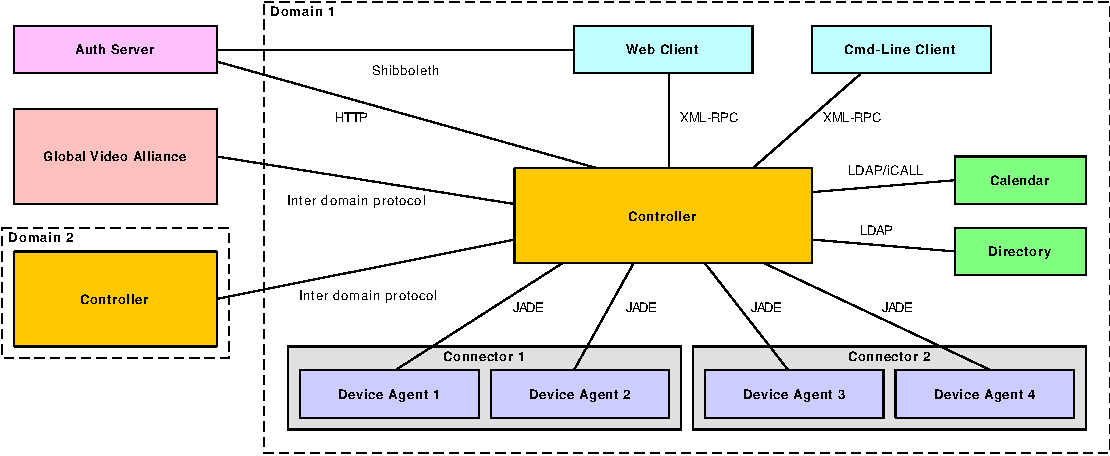
\includegraphics[width=\textwidth]{diagrams/dd_architecture}
\caption{Architecture of Shongo reservation system}
\label{fig:architecture}
\end{figure}

Shongo isn't currently fully implemented. In the current state each Shongo instance is able to manage resources in a single domain without the inter-domain collaboration. The Shongo instance means deployed controller, web client and one or more connectors with one or more device agents. The fig. \ref{fig:architecture-implemented} shows which components and communication channels are already implemented.

\begin{figure}[ht!]
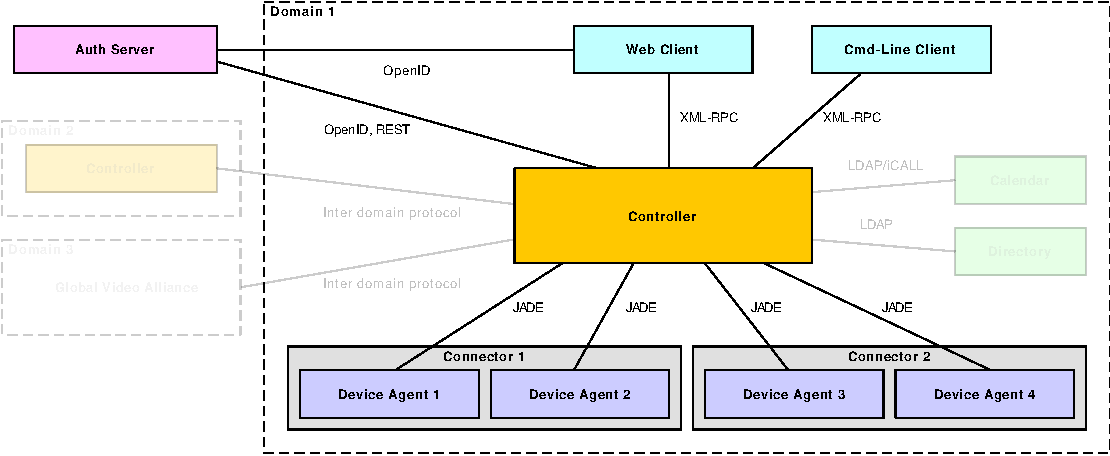
\includegraphics[width=\textwidth]{diagrams/dd_architecture_implemented}
\caption{Already implemented components in Shongo reservation system (grayed parts aren't implemented yet)}
\label{fig:architecture-implemented}
\end{figure}



\chapter{Deployment}

Shongo reservatin system for a single domain can be deployed to target machines in several ways (see fig. \ref{fig:deployment}).

\begin{figure}[ht!]
\begin{center}  
  \subfigure[All components are deployed to the same machine]{
    \label{fig:deployment:one}
    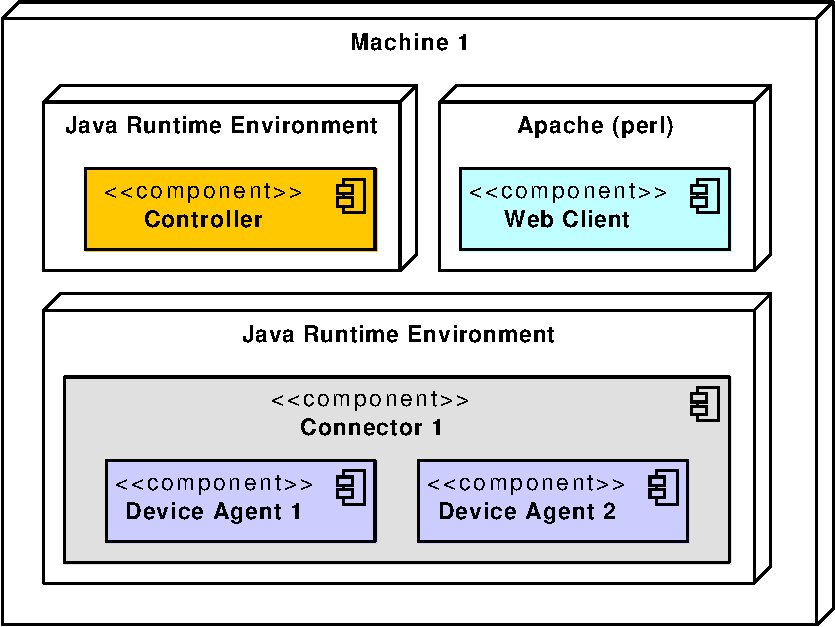
\includegraphics[width=7.5cm]{diagrams/dd_deployment_one}
  } 
  \hfill
  \subfigure[Controller and web client are deployed to the same machine and connector is deployed to another one]{
    \label{fig:deployment:two}
    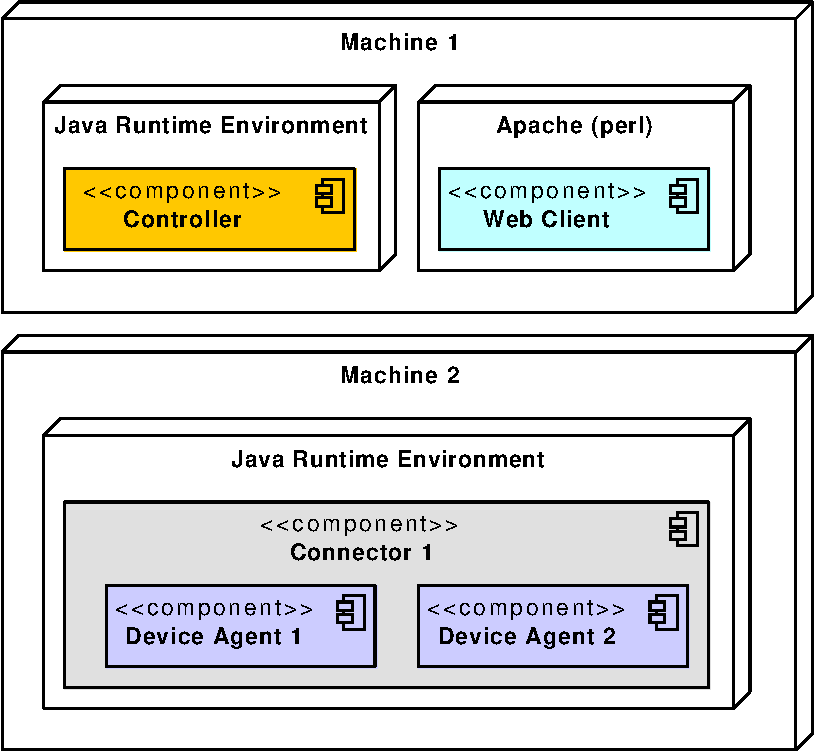
\includegraphics[width=7.5cm]{diagrams/dd_deployment_two}
  } 
  \subfigure[Each component is deployed to it's own machine]{
    \label{fig:deployment:multi}
    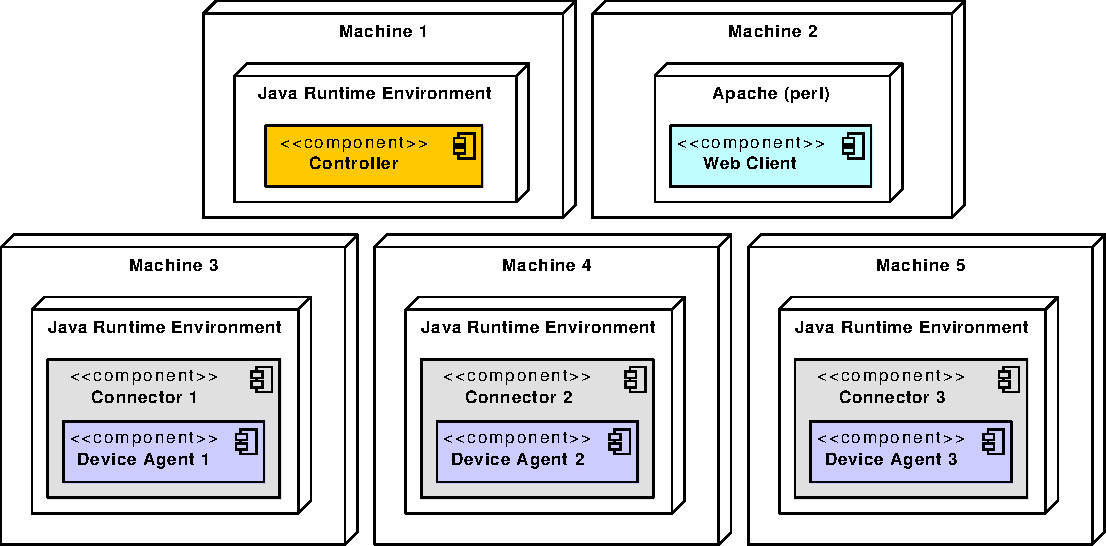
\includegraphics[width=14cm]{diagrams/dd_deployment_multi}
  } 
\end{center}
\caption{Possible deployments of Shongo reservation system components}
\label{fig:deployment}
\end{figure}



\chapter{Controller Relational Database} 

\section{Resources}

\begin{figure}[ht!]
\centering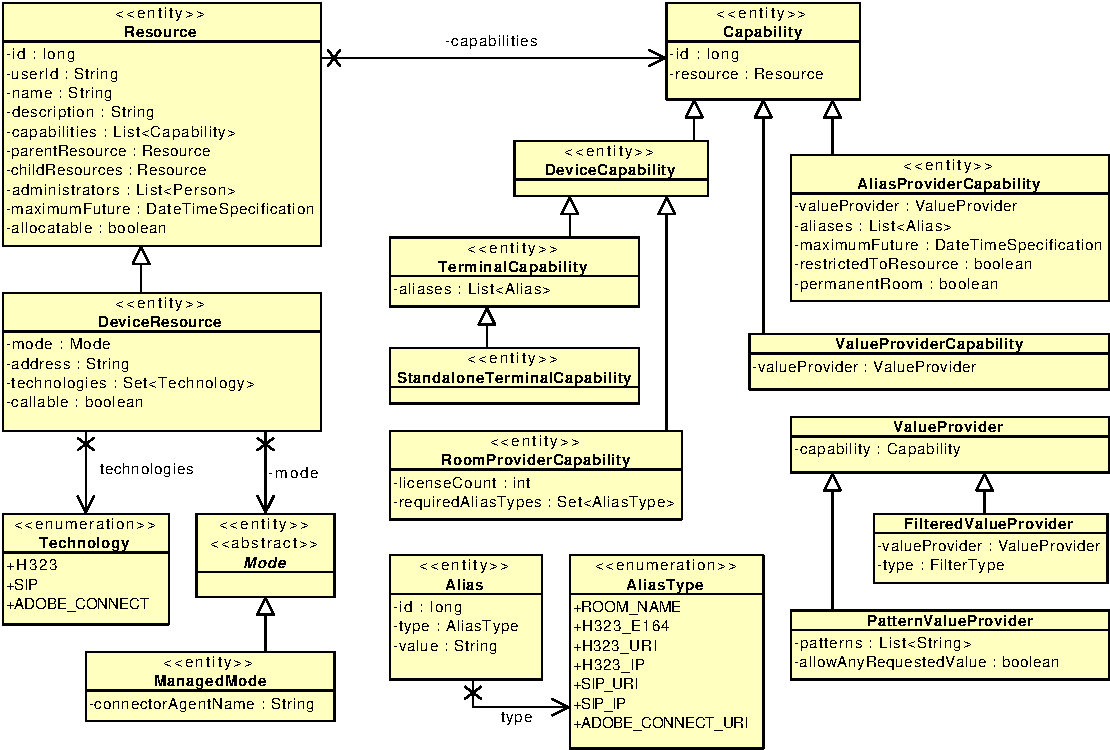
\includegraphics[width=0.8\textwidth]{diagrams/cd_resources}
\caption{Schema of resource database}
\label{fig:resources}
\end{figure}

\begin{itemize}
\item Terminal
\item Multipoint Devices
\item Other
\end{itemize}

\section{Reservation Requests}

\begin{figure}[ht!]
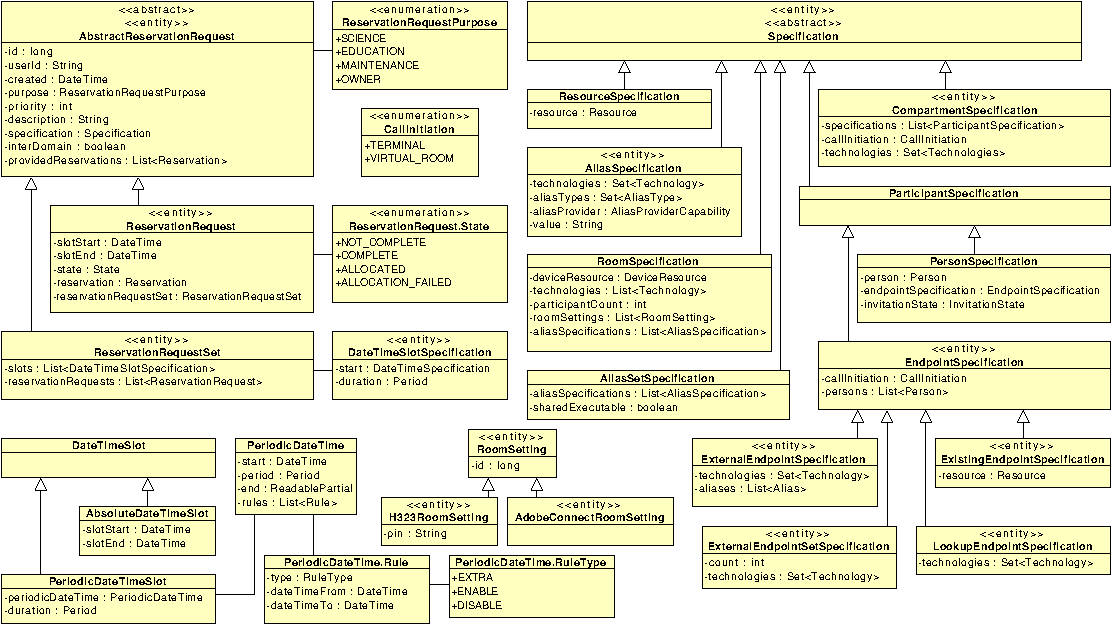
\includegraphics[width=\textwidth]{diagrams/cd_reservation_requests}
\caption{Schema of reservation requests database}
\label{fig:resources}
\end{figure}

\section{Reservations}

\section{Executables}



\chapter{Communication Examples} 

\section{User Perspective}

\section{Administrator Perspective}

\nocite{*}
\bibliography{../bibliography}

\end{document}

